\section{Alerts}
\index{Automation!alerts|see {Alerts}}\index{Alerts}
Alerts allow the user to tie sources of intelligence (such as periodic scheduled searches) to actions (such as a flow that files a ticket). This can make it much simpler to take automatic action when something of interest occurs; rather than defining multiple flows which each run a query and send an email if there are results, you can define a single flow which sends an email, then trigger it with any one of many scheduled searches.

Some basic terminology:

\begin{itemize}
  \tightlist
  \item \emph{Events} are the actual bits of actionable information, for instance ``A user signed in from outside the US''.
  \item \emph{Dispatchers} generate events. A typical dispatcher would be a scheduled search that runs every hour looking for ``bad'' activity; every result returned by a scheduled search is considered an event.
  \item \emph{Consumers} process and respond to events. A typical consumer would be a flow that sends an email to an administrator, or opens a ticket in the ticketing system. Each consumer runs once per event.
  \item \emph{Alerts} tie dispatchers to consumers, ensuring that when a dispatcher generates an event, all associated consumers are executed to process it.
  \item \emph{Schemas} help map the output of dispatchers to consumers by defining fields which are expected in every event.
\end{itemize}

In brief, dispatchers send events, which are then processed by consumers. Events are also ingested into Gravwell under a user-defined tag as a permanent record.

Alerts are managed from the Alerts page, found in the Automations sub-menu.

\subsection{Creating Alerts}
New alerts are created from the Alerts page by clicking the `Create an Alert' icon in the upper right corner. This will open a wizard to define the new alert, as seen in Figure \ref{fig:newalert}

\begin{figure}
	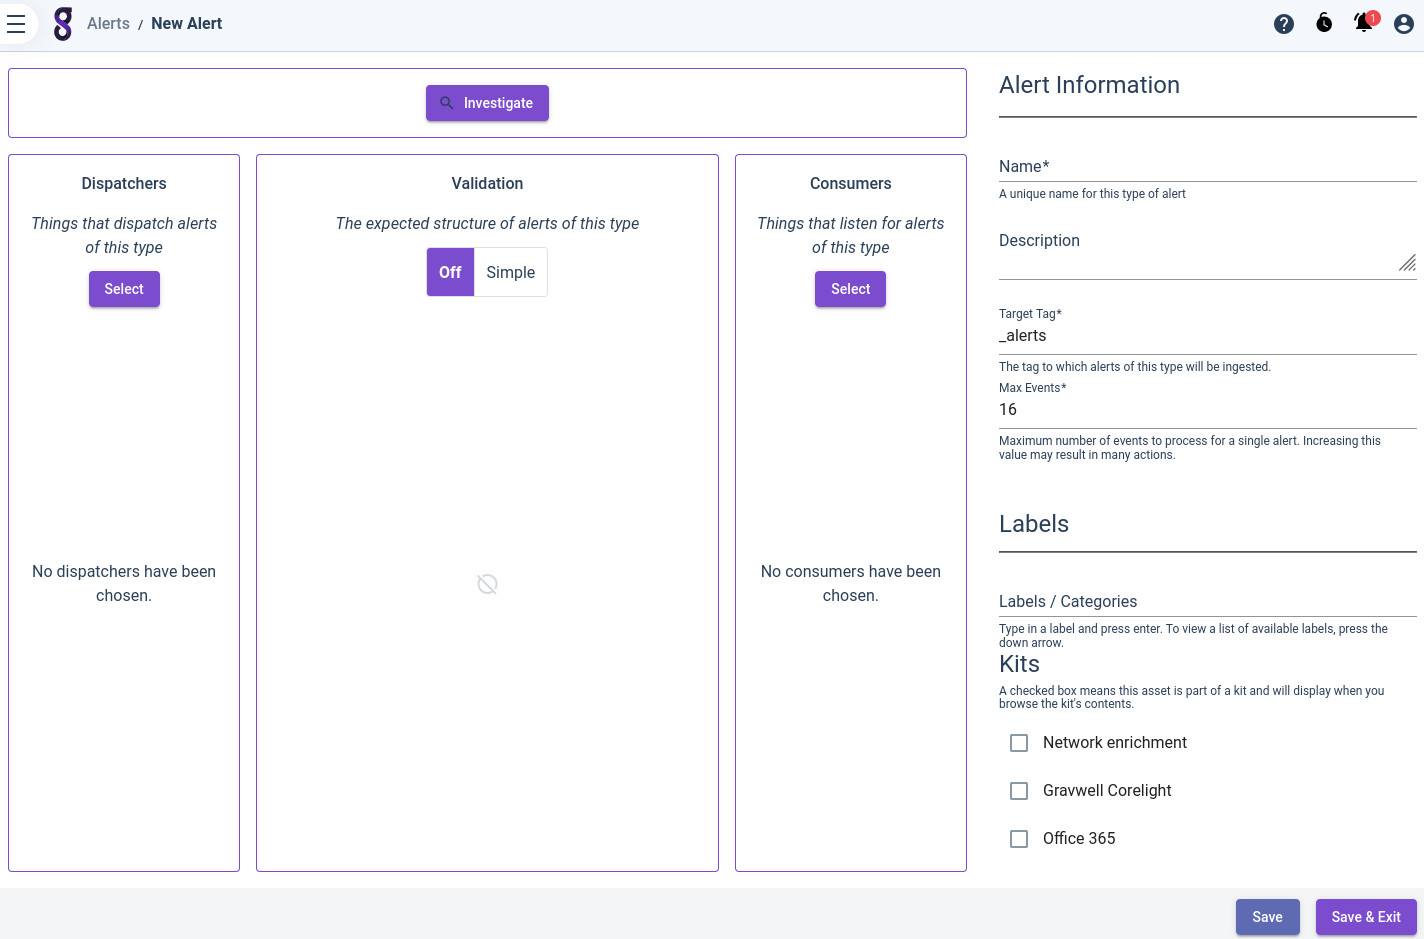
\includegraphics[width=0.85\linewidth]{images/newalert.png}
	\caption{The new alert wizard.}
	\label{fig:newalert}
\end{figure}

The three columns (Dispatchers, Validation, Consumers) reflect the flow of events in an alert: dispatchers generate events, which are (optionally) checked against the schema defined in the Validation column, then finally processed by the consumers.

The Alert Information section on the right should be largely familiar, as most of the fields are the same as in other wizards throughout Gravwell. However, the Target Tag and Max Events parameters are specific to alerts and deserve explanation.

\subsubsection{Target Tag}
The Target Tag parameter defines which tag will receive events and logs for this alert. In general, we recommend the following best practices:

\begin{itemize}
  \tightlist
  \item Use a unique tag for each alert.
  \item Use the same prefix on all alert tags (e.g. \code{\_alerts}) to more easily query *all* alerts at once.
\end{itemize}

\subsubsection{Max Events}

The Max Events parameter controls how many events will be processed from any given dispatcher. For instance, if one dispatcher is a query which may return hundreds of results, but you have set Max Events to 10, only 10 of the results will be taken as events for each run of the dispatcher.

Max Events is an important safeguard against accidentally creating hundreds of tickets or sending thousands of emails; although your dispatcher may generally return only a few results (or no results), if a new data source is added to Gravwell it may suddenly start returning hundreds of results!

Max Events can be any integer from 0 to 8192. Setting it to 0 is equivalent to specifying the max. If you find yourself needing more than 8192 events per dispatcher run, it may be time to consider a dedicated flow or an external script instead.

\subsection{Defining Dispatchers}
Dispatchers are scheduled searches. When a scheduled search runs and returns a non-zero number of results, Gravwell checks to see if any alerts have that search set as a dispatcher. If so, Gravwell fetches results from the scheduled search, adds some event metadata to each, and sends them to the consumers.

Scheduled searches can be attached to alerts as dispatchers in two ways. The first option is by clicking `Select' in the Dispatchers column of the alert editor (Figure \ref{fig:dispatchers-select}). The second option is through the scheduled search editor, as seen in Figure \ref{fig:scheduled-dispatch}.

\begin{figure}
	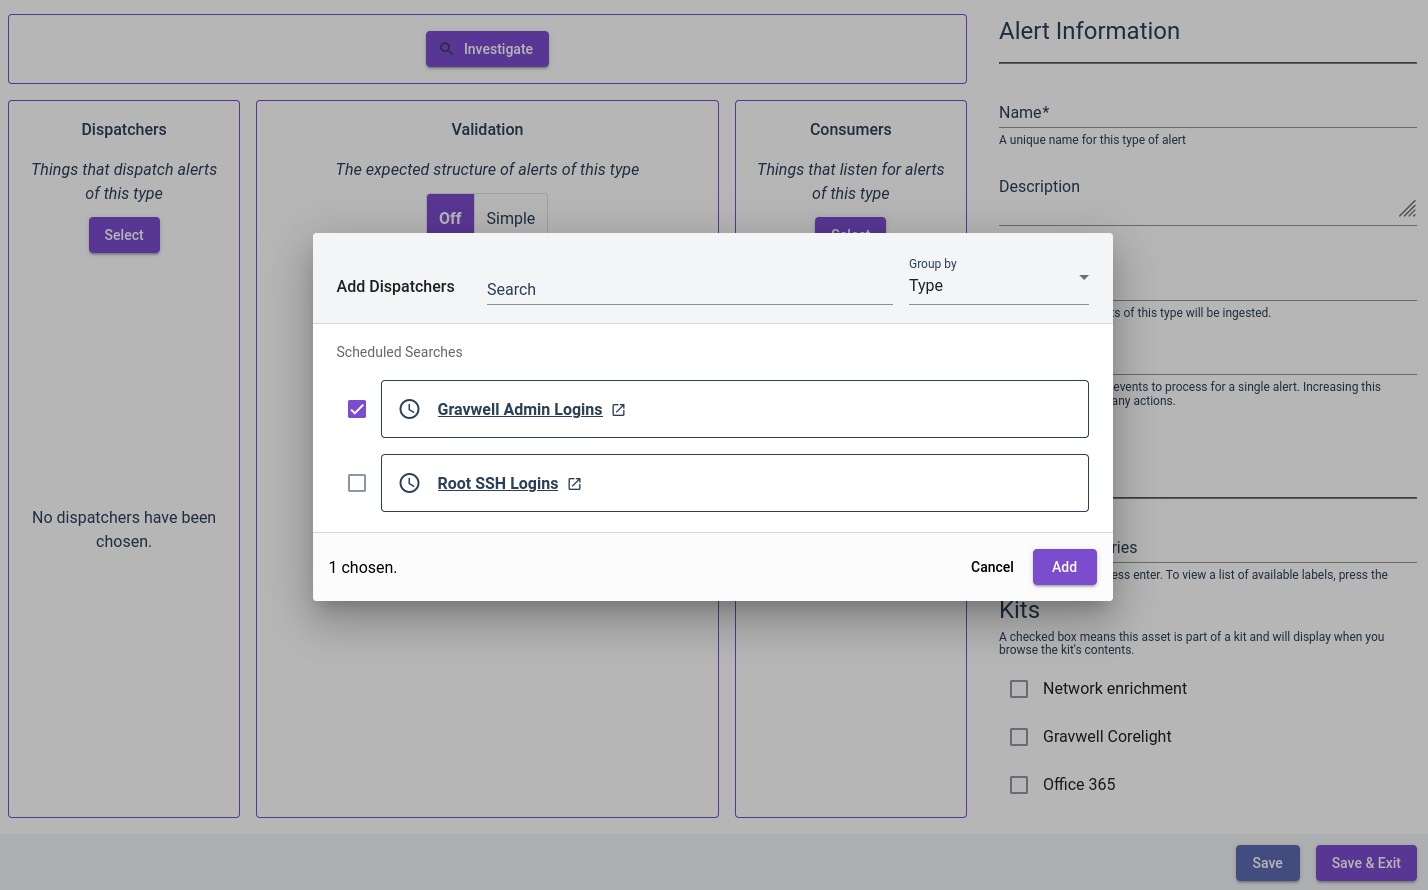
\includegraphics[width=0.85\linewidth]{images/dispatchers-select.png}
	\caption{Selecting dispatchers from within the alert editor.}
	\label{fig:dispatchers-select}
\end{figure}

\begin{figure}
	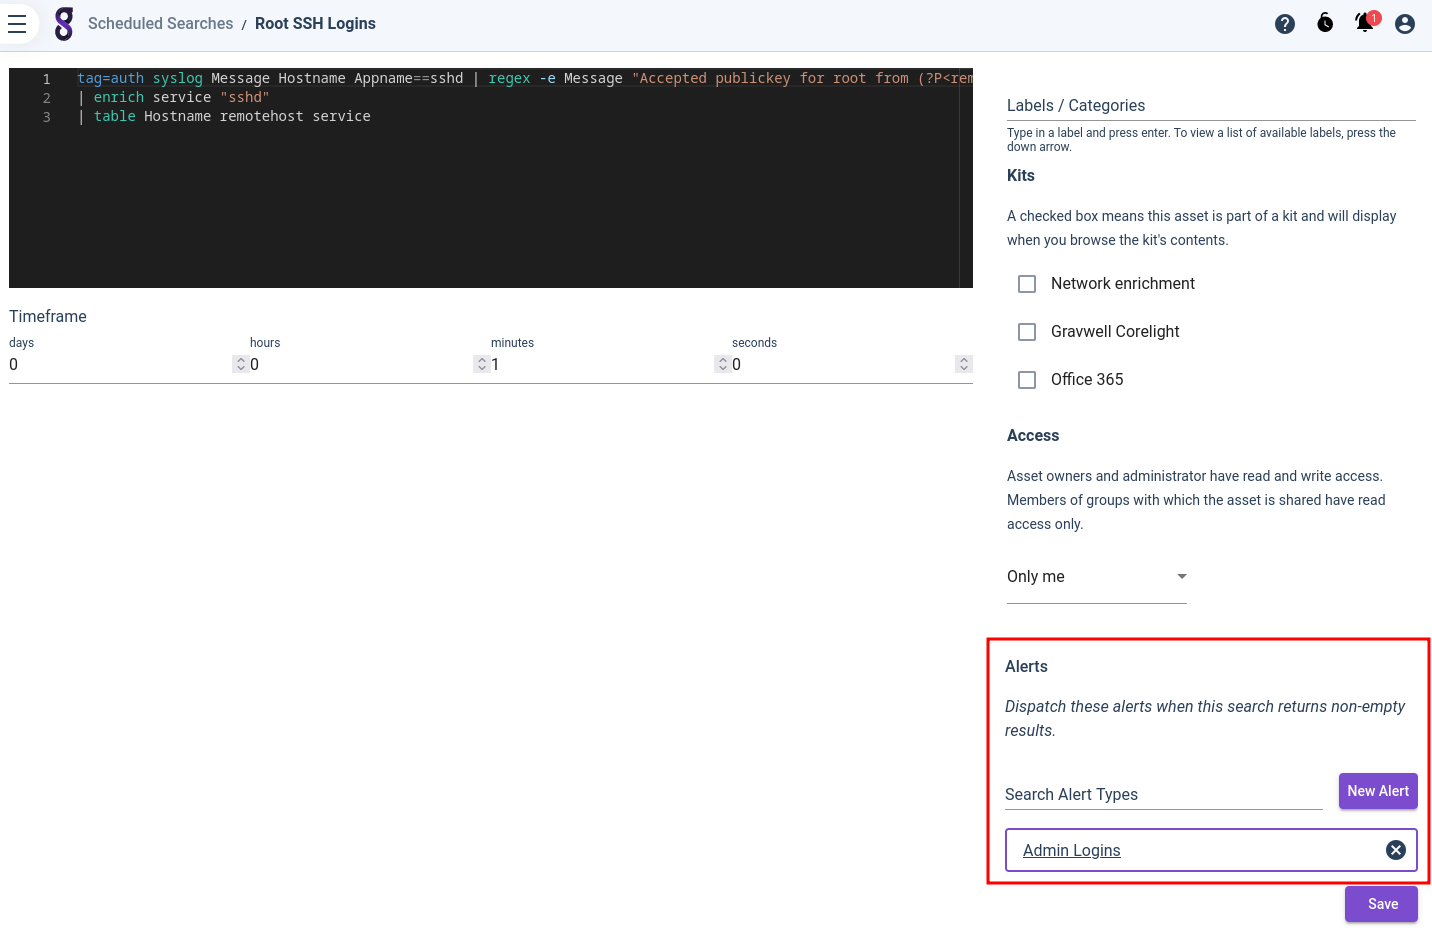
\includegraphics[width=0.85\linewidth]{images/scheduled-dispatch.png}
	\caption{Adding a scheduled search to an alert from the scheduled search editor.}
	\label{fig:scheduled-dispatch}
\end{figure}

There are a few key things to consider when defining scheduled searches to use as dispatchers:

\begin{itemize}
  \tightlist
\item Use only the \code{text/raw} or \code{table} renderers.
\item Every result will be an individual event; consider using the stats modules to ``summarize'' your results when there is a lot of data.
\item If you're going to attach multiple dispatchers to one alert, try to use the same set of enumerated value names in all dispatchers (see section \ref{sec:alert-schemas} for further discussion).
\end{itemize}

\clearpage
\subsection{Defining Schemas}
\label{sec:alert-schemas}
Schemas help the user ensure that their dispatchers emit events in a format their consumers expect. By defining a schema on an alert, the user declares that they expect all dispatchers to include certain fields in their results; consumers may then operate on the assumption that those fields will exist in each event. Although defining a schema for an alert is optional, it is highly recommended.

Schemas are defined using the \emph{Validation} section of the alert editor. Figure \ref{fig:alert-schema} shows an example in which three fields have been defined: ``Hostname'', ``remotehost'', and ``service'', all strings. The two dispatchers in the left column must emit these fields, either as enumerated values on the results (when the text renderer is used) or as columns in a table (when using the table renderer).

\begin{figure}
	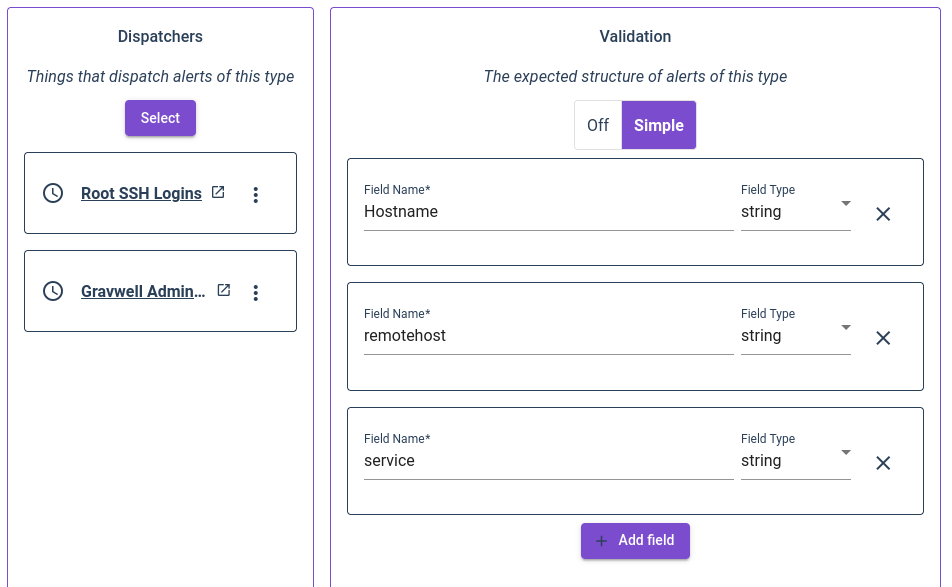
\includegraphics[width=0.8\linewidth]{images/alert-schema.png}
	\caption{Defining an alert schema.}
	\label{fig:alert-schema}
\end{figure}

If a dispatcher does \emph{not} output all the fields in the schema, warnings will be displayed, as seen in Figure \ref{fig:schema-warning}, where an additional field ``foo'' has been added.

\begin{figure}
	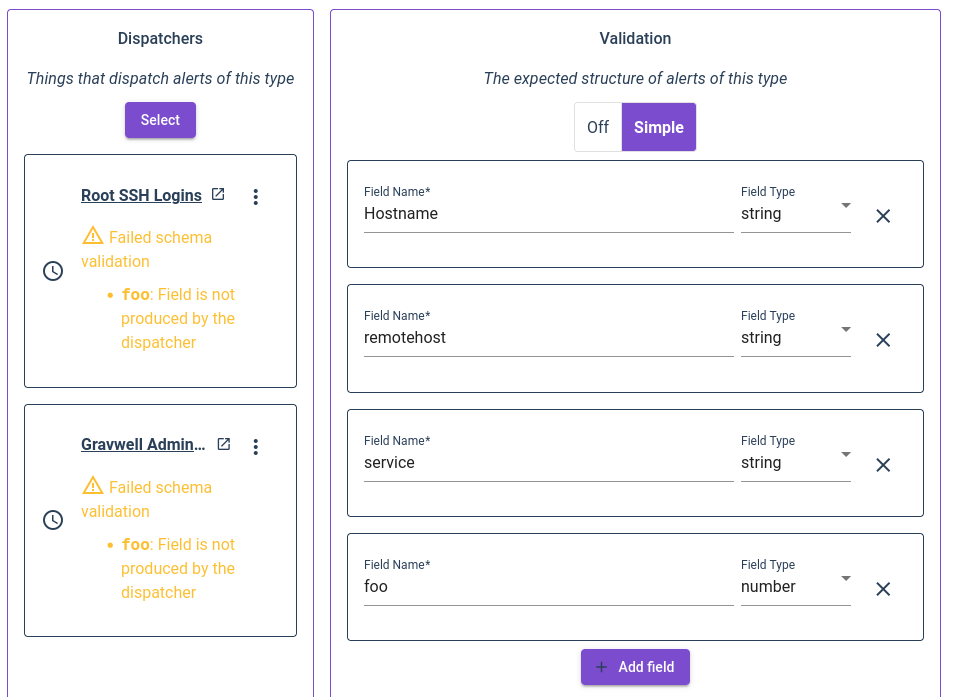
\includegraphics[width=0.8\linewidth]{images/schema-warning.png}
	\caption{Warnings due to mismatched schema and dispatchers.}
	\label{fig:schema-warning}
\end{figure}

\clearpage
\subsection{Defining Consumers}
Currently, flows are the only type of consumers supported for alerts. When a flow executes as a consumer, the incoming payload contains an additional item named event which contains the event sent by the dispatcher. Refer to section \ref{sec:flows} for further discussion of flows.

To build a flow as a consumer, create the flow, then associate it with the alert in the Settings tab as seen in Figure \ref{fig:flow-alert}. Once the flow is associated, the debug context dropdown menu in the Flow Designer tab will list the associated alert (Figure \ref{fig:flow-context}); selecting the alert will make debug runs of the flow behave \emph{as though triggered by that alert}. Specifically, the flow editor will generate a ``sample'' event which is passed in to the flow during the debug run. Note that this sample event uses auto-generated values; clicking the pencil icon to the right of the debug context dropdown will open a dialog in which you may edit the sample event if you wish (see Figure \ref{fig:context-edit}, in which the ``service'' field has already been changed).

\begin{figure}
	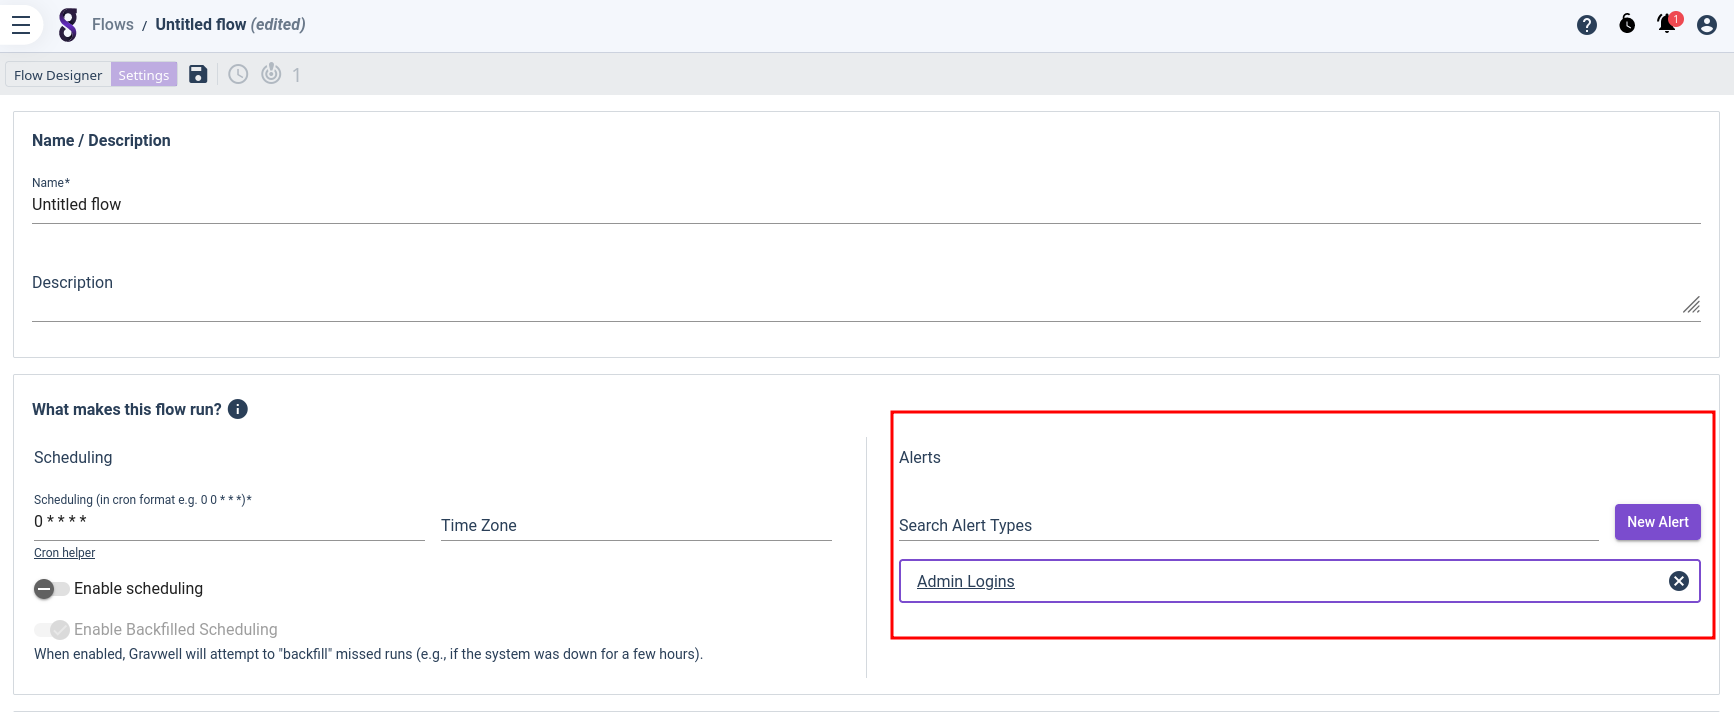
\includegraphics[width=0.8\linewidth]{images/flow-alert.png}
	\caption{Associating a flow with an alert.}
	\label{fig:flow-alert}
\end{figure}

\begin{figure}
	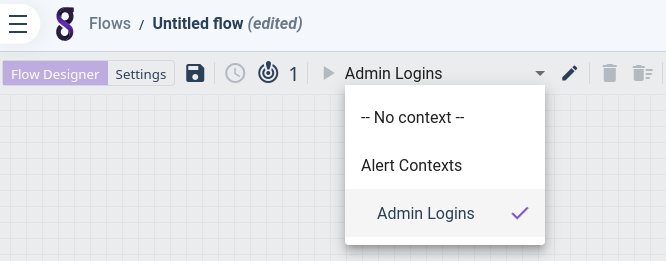
\includegraphics[width=0.8\linewidth]{images/flow-context.png}
	\caption{Selecting flow debug context.}
	\label{fig:flow-context}
\end{figure}

\begin{figure}
	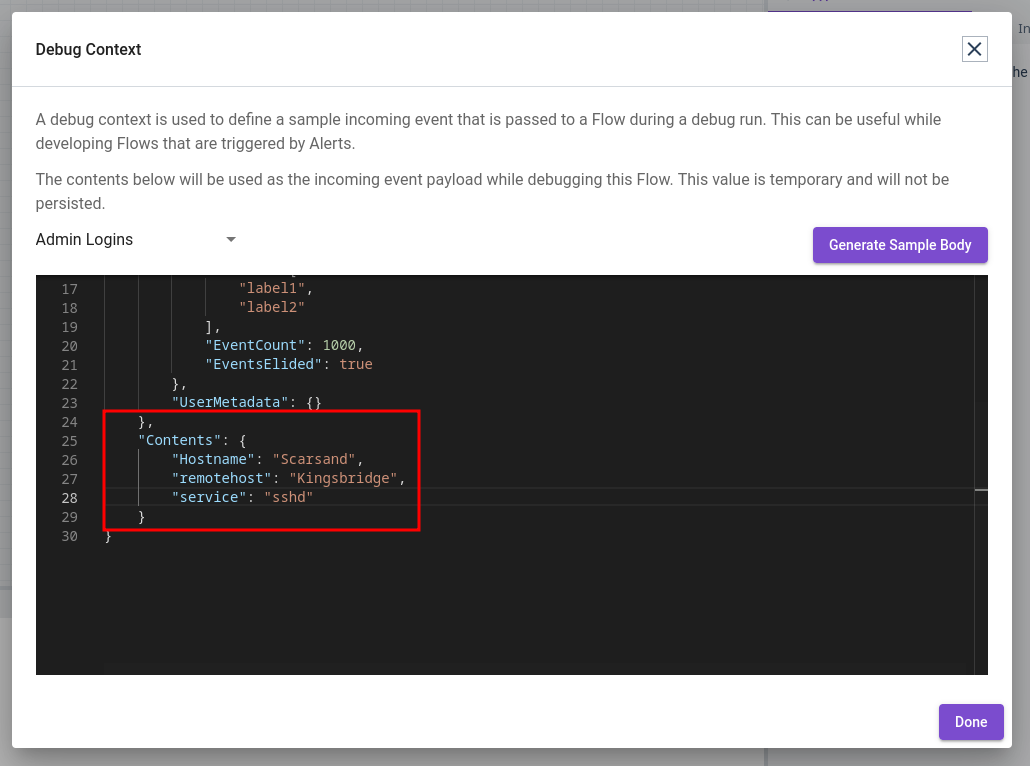
\includegraphics[width=0.8\linewidth]{images/context-edit.png}
	\caption{Editing flow debug context.}
	\label{fig:context-edit}
\end{figure}

The contents of this sample event are injected into the incoming flow payload under the name \code{event}; when the alert is actually activated, the real events will be injected in the same way.

A simple consumer flow could use Text Template nodes to build a subject line and body for an email, then use the Email node to actually send the mail. Figures \ref{fig:template-subject} and \ref{fig:template-body} show how the fields of the \code{event} are referenced in the template node; Figure \ref{fig:email-consumer} then shows how the Email node uses the results to send a message.

\begin{figure}
	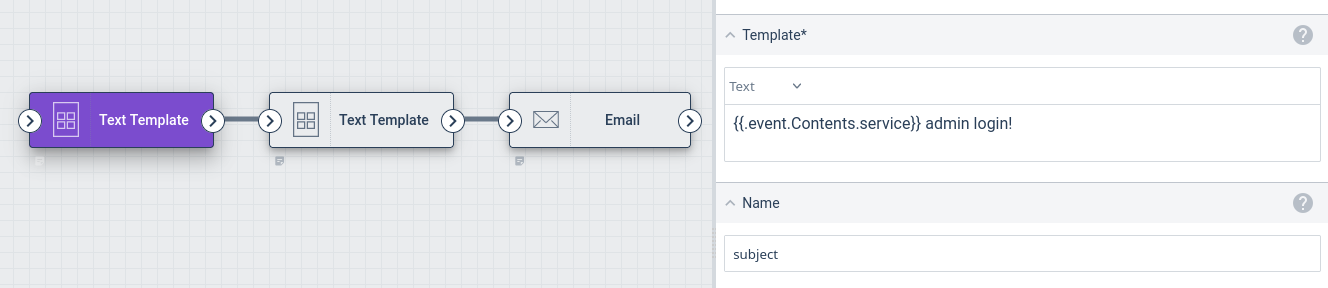
\includegraphics[width=0.85\linewidth]{images/template-subject.png}
	\caption{Building a subject line from an event.}
	\label{fig:template-subject}
\end{figure}

\begin{figure}
	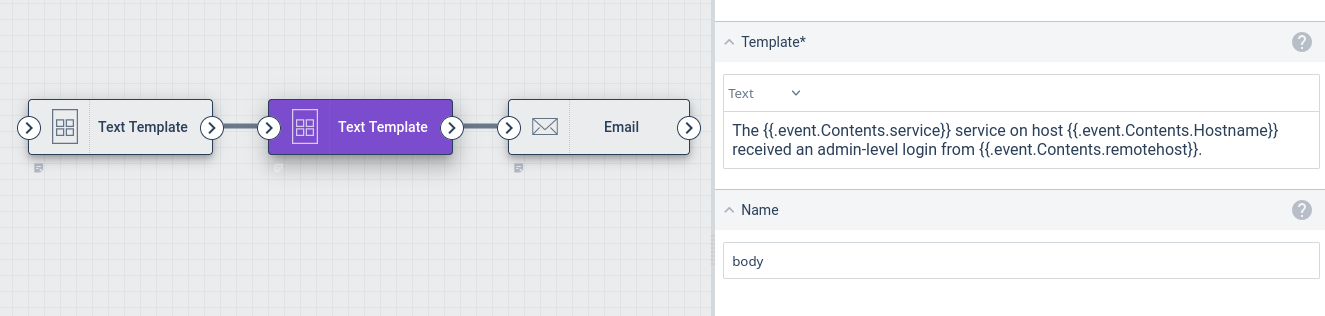
\includegraphics[width=0.85\linewidth]{images/template-body.png}
	\caption{Building a message body from an event.}
	\label{fig:template-body}
\end{figure}

\begin{figure}
	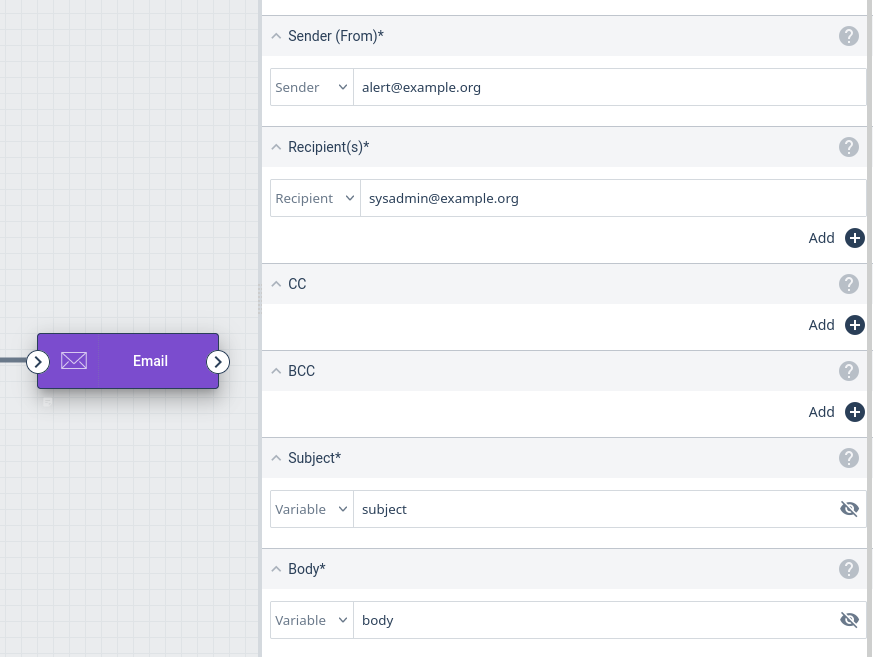
\includegraphics[width=0.75\linewidth]{images/email-consumer.png}
	\caption{Sending an email in an alert consumer.}
	\label{fig:email-consumer}
\end{figure}

\clearpage
\subsection{Hands-on Lab}
This lab will demonstrate how to build a simple alert. In the hands-on lab of the flows section (\ref{sec:flow-lab}), we used a flow to run a query looking for failed logins, then set a notification if any were detected. In this lab, we will create an alert with similar behavior and explore the extra flexibility alerts give us. First, create a Gravwell webserver+indexer container:

\begin{Verbatim}[breaklines=true]
docker run -d --rm --net gravnet -p 8080:80 --name gravwell gravwell:base
\end{Verbatim}

Now log into the web GUI (\href{http://localhost:8080}{http://localhost:8080}). Then, open a new \emph{private} browser window (so the existing login cookie isn't used), go to the same GUI URL, and enter some invalid login credentials, e.g. username ``admin'' with password ``admin''. This will generate a login failure message which we can check using the following query:

\begin{Verbatim}[breaklines=true]
tag=gravwell syslog Message=="Authentication failure" user 
| stats count by user 
| table user count
\end{Verbatim}

Create a new scheduled search containing that query which runs over the last \emph{minute} of data every minute, as seen in Figure \ref{fig:alert-lab-search}.

\begin{figure}
	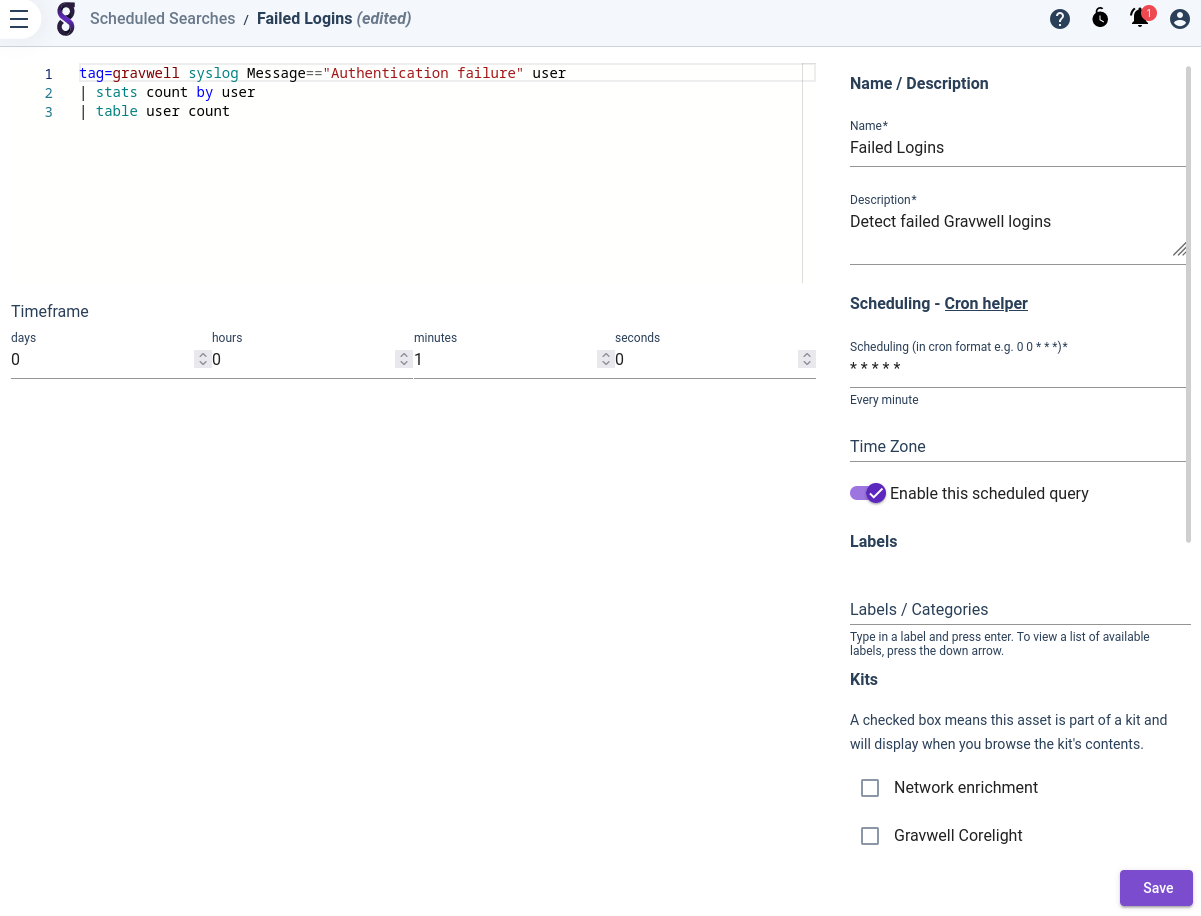
\includegraphics[width=0.85\linewidth]{images/alert-lab-search.png}
	\caption{Defining a scheduled search dispatcher for failed logins.}
	\label{fig:alert-lab-search}
\end{figure}

Next, create an alert which uses the previously-defined scheduled search as a dispatcher. Define a validation schema which expects a field named ``user''; for our purposes, we don't necessarily need the ``count'' field from the search, so we can omit it. Ingest it into the tag \code{\_alerts\_logins} and set Max Events to 16. Figure \ref{fig:alert-lab-alert} shows how your alert should look.

\begin{figure}
	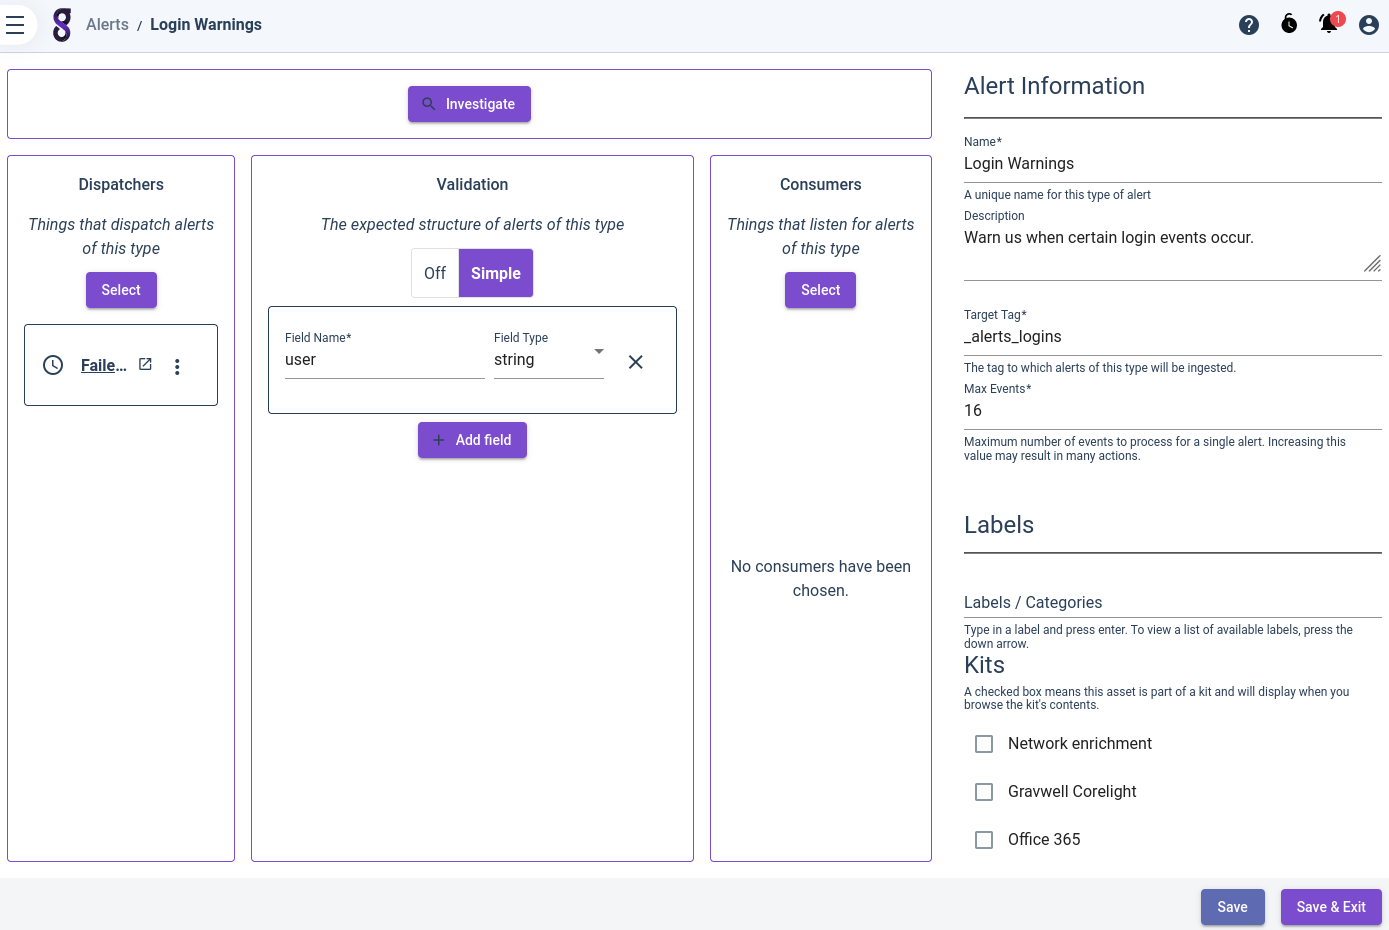
\includegraphics[width=0.85\linewidth]{images/alert-lab-alert.png}
	\caption{Defining an alert.}
	\label{fig:alert-lab-alert}
\end{figure}

Finally, we'll create a very simple flow which just alerts the user that \emph{something} has occurred. The flow should have only a Gravwell Notification node with the message set to something like ``Login problems! Check \_alerts\_logins tag'' (Figure \ref{fig:alert-lab-flow}. In the flow settings, link it with the alert we defined earlier.

\begin{figure}
	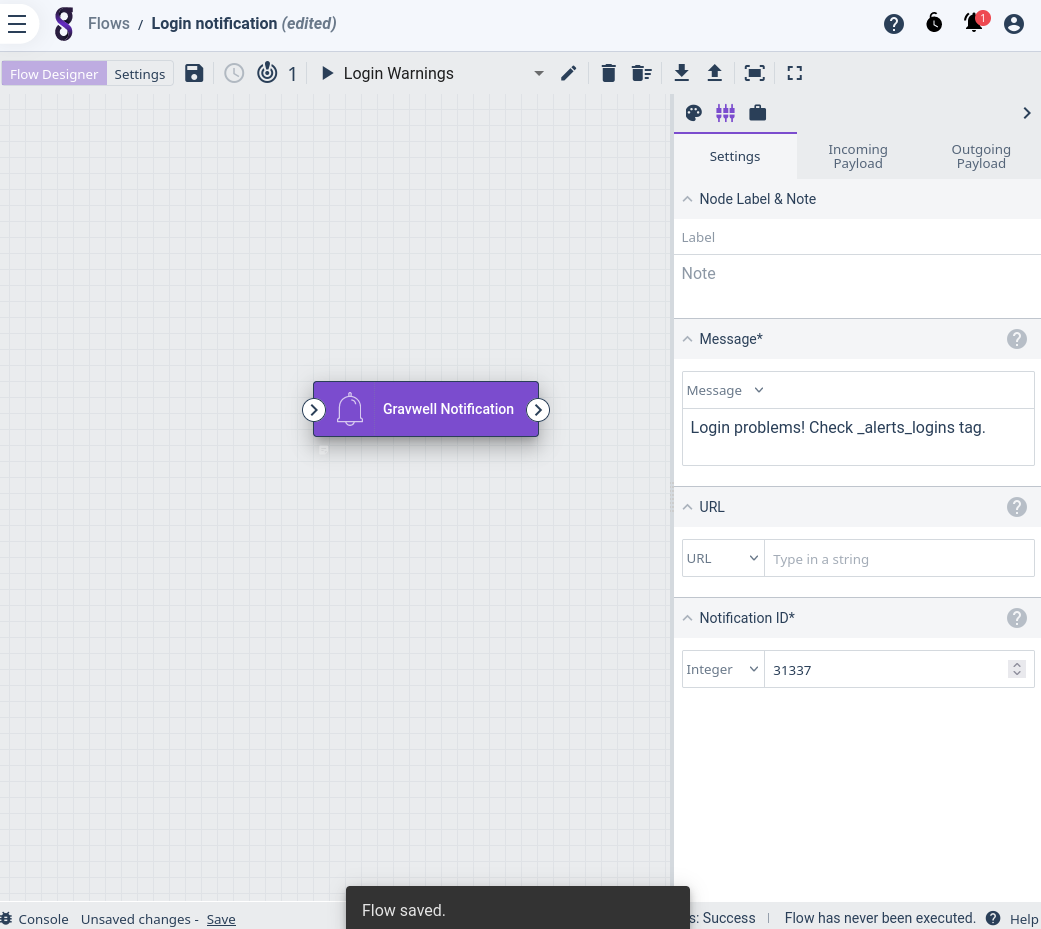
\includegraphics[width=0.85\linewidth]{images/alert-lab-flow.png}
	\caption{Defining a consumer flow.}
	\label{fig:alert-lab-flow}
\end{figure}

To test the alert, open another private window, go to the Gravwell URL (\href{http://localhost:8080}{http://localhost:8080}), and enter some invalid login credentials again. You'll have to wait until the start of the next minute, when the scheduled search executes, to verify; at that point, you should see a new notification informing you that login problems have occurred. You can then open the Query Studio and run a search to see the ingested alert:

\begin{Verbatim}[breaklines=true]
tag=_alerts_logins
\end{Verbatim}

Note that the ingested events have \emph{lots} of metadata associated with them, such as which scheduled search created the event, which alert received it, etc.

\subsubsection{Questions/Exercises}

\begin{enumerate}
\item The scheduled search runs over only the most recent 1 minute of logs, but the notification persists once set until you clear it. Why?
\item What will happen if there are dozens of failed logins in a single minute?
  \begin{enumerate}
  \item How many events will be ingested each time?
  \item How could we change that number?
  \item How could we adjust the search to reduce the number of events ingested?
  \end{enumerate}
\item Add another dispatcher which will fire whenever the admin user logs in \emph{successfully} -- many organizations like to monitor when privileged accounts are accessed! Test it by logging in as admin with the correct credentials. (Hint: \code{tag=gravwell syslog Message=="User logged in" user==admin} will find successful admin logins)
  \begin{enumerate}
  \item Does the new query match the schema we defined? Why/why not?
  \end{enumerate}
\end{enumerate}

To clean up after the experiment, run:

\code{docker kill \$(docker ps -a -q)}
